% This is LLNCS.DEM the demonstration file of
% the LaTeX macro package from Springer-Verlag
\documentclass[a4paper,12pt]{llncs}
%
\usepackage{makeidx}  % allows for indexgeneration
\makeindex

\usepackage[ngerman]{babel}
\usepackage[utf8]{inputenc}      % Code-Page latin 1
\usepackage[T1]{fontenc}
% Nur eine der beiden folgenden Zeilen einbinden!
% siehe Abschnitt Bilder
%\usepackage{graphicx}       % Bilder einbinden, Version fuer normales latex
\usepackage[pdftex]{graphicx}       % Bilder einbinden, Version fuer pdflatex

% mit Hyperrefs
\usepackage[pdftex, plainpages=false,hypertexnames=true,pdfnewwindow=true,backref=true,colorlinks=true,citecolor=blue,linkcolor=black,urlcolor=blue,filecolor=blue]{hyperref}% 
% weitere Packages
\usepackage{ifthen}                 % Zum Auskommentieren von Textteilen
\usepackage{amssymb}                % Mathematische Buchstaben
\usepackage{amsmath}                % Verbesserter Formelsatz
\usepackage[vlined,boxed]{algorithm2e}
\usepackage{booktabs}               % schönere Tabellen
\usepackage{color}
\usepackage{hyperref}
 \hypersetup{urlcolor=black,citecolor=black}
%\setalcapskip{1.5ex} % fuer package algorithm
\usepackage{dsfont}  
%\newtheorem{definition}{Definition}
\usepackage{doc}
\usepackage{listings}
\usepackage{subcaption}
\usepackage{url}

% Seitenformat ===============================================================
\hoffset=-1.25truecm
\setlength{\topmargin}{0.0cm}
\setlength{\textheight}{23.0cm}
\setlength{\footskip}{1.5cm}
\setlength{\textwidth}{15.4cm}
\setlength{\evensidemargin}{1.5cm}
\setlength{\oddsidemargin}{1.5cm}
\setlength{\parskip}{1ex}
\setlength{\parindent}{0pt}
\setlength{\marginparwidth}{1.4cm}
\setlength{\marginparsep}{1mm}
\setalcapskip{1.5ex} % fuer package algorithm

\pagestyle{plain}

% Makro-Definitionen ==========================================================
% Zahlenbereiche -------------------------------------------------------------
\newcommand{\N}{{\mathbb{N}}}
\newcommand{\R}{{\mathbb{R}}}
\newcommand{\C}{{\mathbb{C}}}
\newcommand{\Z}{{\mathbb{Z}}}
\newcommand{\Q}{{\mathbb{Q}}}

\renewcommand{\lstlistingname}{Auflistung}

\makeatletter
\newcommand\nocaption{%
	\renewcommand\p@subfigure{}
	\renewcommand\thesubfigure{\thefigure\alph{subfigure}}
}
\makeatother
% 
\def\myverzeichnis{.}

\numberwithin{equation}{section} 
% Bild -----------------------------------------------------------------------
% #1 Filename;  #2 Label;  #3 Bildunterschrift;  #4 Kurzform
\newcommand{\bild}[4]{
  \begin{figure}[htbp]
    \begin{center}
      \includegraphics{#1}
      \caption[#4]{#3}
      \label{#2}
    \end{center}
  \end{figure}
}

% Bildbreite -----------------------------------------------------------------
% #1 Filename;  #2 Breite;  #3 Label;  #4 Bildunterschrift;  #5 Kurzform
\newcommand{\bildbreite}[5]{
  \begin{figure}[htbp]
    \begin{center}
      \includegraphics[width=#2]{#1}
      \caption[#5]{#4}
      \label{#3}
    \end{center}
  \end{figure}
}

% !TeX spellcheck = de_DE
% ============================================================================
\begin{document}

% =========== Das war der Vorspann, jetzt geht's los! ========================

% ============================================================================
% =============  AB HIER DARF UND SOLL GETIPPT WERDEN ========================
% ============================================================================

\author{Yaroslav Nalivayko}
\index{Yaroslav Nalivayko}

% Das Institut wird fuer den Betreuer missbraucht ...
\institute{{\bf Betreuer:} M.Sc. Benjamin Maier}
\authorrunning{Yaroslav Nalivayko}
\title{Newton-Fraktale}

\maketitle

\thispagestyle{empty}

\begin{abstract}
%In dieser Arbeit werden Newton-Fraktale behandelt.
Wenn man das Newton-Verfahren für die Lösung der nichtlinearen Gleichungen auf der komplexen Ebene einsetzt und versucht die Ergebnisse zu visualisieren, erscheinen sehr interessante Figuren, die eine selbstähnliche Struktur besitzen.
Solche Figuren heißen Newton-Fraktale, die in dieser Arbeit behandelt werden.
Es werden Ursachen für ihre Struktur benannt und manche Beispiele analysiert. 
%die sind die Teilmenge der mathematischen Fraktale, die durch die Einsetzung des Newton-Verfahrens für die Lösung der nichtlinearen Gleichungen auf der komplexen Ebene erscheinen.
\end{abstract}

% Einleitung -----------------------------------------------------------------
\section{Einleitung}
Newton-Fraktale stellen eine interessante Klasse der mathematischen Fraktale dar. 
Im Rahmen dieser Arbeit werden theoretische Grundlagen vorgestellt und wird ein Programm für die \nameref{sec:vis} der Fraktalen entwickelt.
In der letzten Sektion findet die \nameref{sec:analy} mancher interessanten Funktionen statt.


\section{Theoretische Grundlagen}\label{sec:theo}
Hier werden wichtigste Grundbegriffe erläutert. 
Der Anwendungsgebiet der numerischen Mathematik wird gezeigt.
Das Arbeitsprinzip des Newtonverfahrens wird aufklärt und veranschaulicht.
Dann werden natürliche und künstliche Fraktale vorgestellt und Newton-Fraktale präsentiert.

\subsection{Numerische Mathematik}
Die numerische Mathematik beschäftigt sich als Teilgebiet der Mathematik mit der Konstruktion und Analyse von Algorithmen für kontinuierliche mathematische Probleme.~\cite{nummath}
Sie wird oft benutzt, um approximative Lösungen mit Hilfe des Rechners zu finden.
Im Vergleich zu analytischen Lösungen helfen approximative Verfahren nur eine Näherung der Lösung zu finden.
Gewöhnlich haben diese Methoden eine iterative Form, das heißt, dass nach jedem Iterationsschritt bekommt man eine genauere Lösung.
Numerische Mathematik wird oft benutzt, wenn, zum Beispiel, eine Gleichung schwer zu lösen ist, wenn eine Näherungslösung akzeptabel ist oder wenn man einen Rechner für die Determination der Lösung benutzen will.

\subsection{Newton-Verfahren}
Newton-Verfahren ist das iterative numerische Verfahren, das die Nullstelle gegebener Funktion findet.
Die Methode wurde nach Sir Isaac Newton benannt. \\
Wir interessieren uns für stetig differenzierbare Funktionen mit nur einer Variable.
\[
f(x) = 0
\] 
Man wählt den Startwert $x_0$ manuell und benutzt folgende iterative Methode, bis eine akzeptable Lösung gefunden wird.
\[
x_{n+1} = x_n - \frac{f(x_n)}{f'(x_n)}
\] 
Auf jedem Iterationsschritt wird eine Tangente zu $f(x)$ im Punkt $x_n$ gebildet.
Die Tangente schneidet die x-Achse im Punkt $x_{n+1}$. 
Beispiel auf dem Bild~\ref{fig:newton}.
Das zeigt, dass für eine stetig differenzierbare Funktion das Punkt $x_{n+1}$ näher zu einer Nullstelle als das Punkt $x_n$ liegt.
Nach dem nächsten Iterationsschritt wird das Punkt $x_{n+2}$ berechnet, der noch näher wird.\\
Gewöhnlich wählt man eine zulässige "Fehler" $\varepsilon>0$ und eine maximale Anzahl der Schritte $N$.
Nach jedem Schritt der iterativen Methode prüft man, ob $f(x_n)  < \varepsilon$ ist. 
In diesem Fall ist die Lösung gefunden.
Und falls $n > N$ ist, dann wird die Lösung in der akzeptablen Anzahl der Schritte unauffindbar. 
Iterativer Prozess der Annäherung von $x_n$ zu $x_{n+1}$ heißt Konvergenz, und falls $x_0$ zu $x_n$ kommt, heißt das, dass $x_0$ gegen $x_n$ konvergiert.

\begin{figure}[ht]   
	\centering
	\includegraphics[width=.5\linewidth]{figures/newton}
	\caption{Newton-Verfahren\\\tiny{https://de.wikipedia.org/wiki/Datei:Newtonsches\_N\%C3\%A4herungsverfahren.png}}
	\label{fig:newton}
\end{figure}

\subsection{Fraktale}
Fraktal (lateinisch $fractus$ - gebrochen) ist ein vom Mathematiker Benoît Mandelbrot geprägter Begriff, der bestimmte natürliche oder künstliche Gebilde oder Muster bezeichnet. 
Diese Gebilde oder Muster weisen einen hohen Grad von Skaleninvarianz bzw. Selbstähnlichkeit auf. 
Das ist beispielsweise der Fall, wenn ein Objekt aus mehreren verkleinerten Kopien seiner selbst besteht.~\cite{fraktal} \\
Die Figur \ref{fig:frac_natur} stellt ein Beispiel für ein naturgegebenes Fraktal, und die Figur~\ref{fig:frac_math} für ein mathematisches Fraktal.
\begin{figure}[ht]   
	\nocaption
	\begin{subfigure}{.5\textwidth}
		\centering
		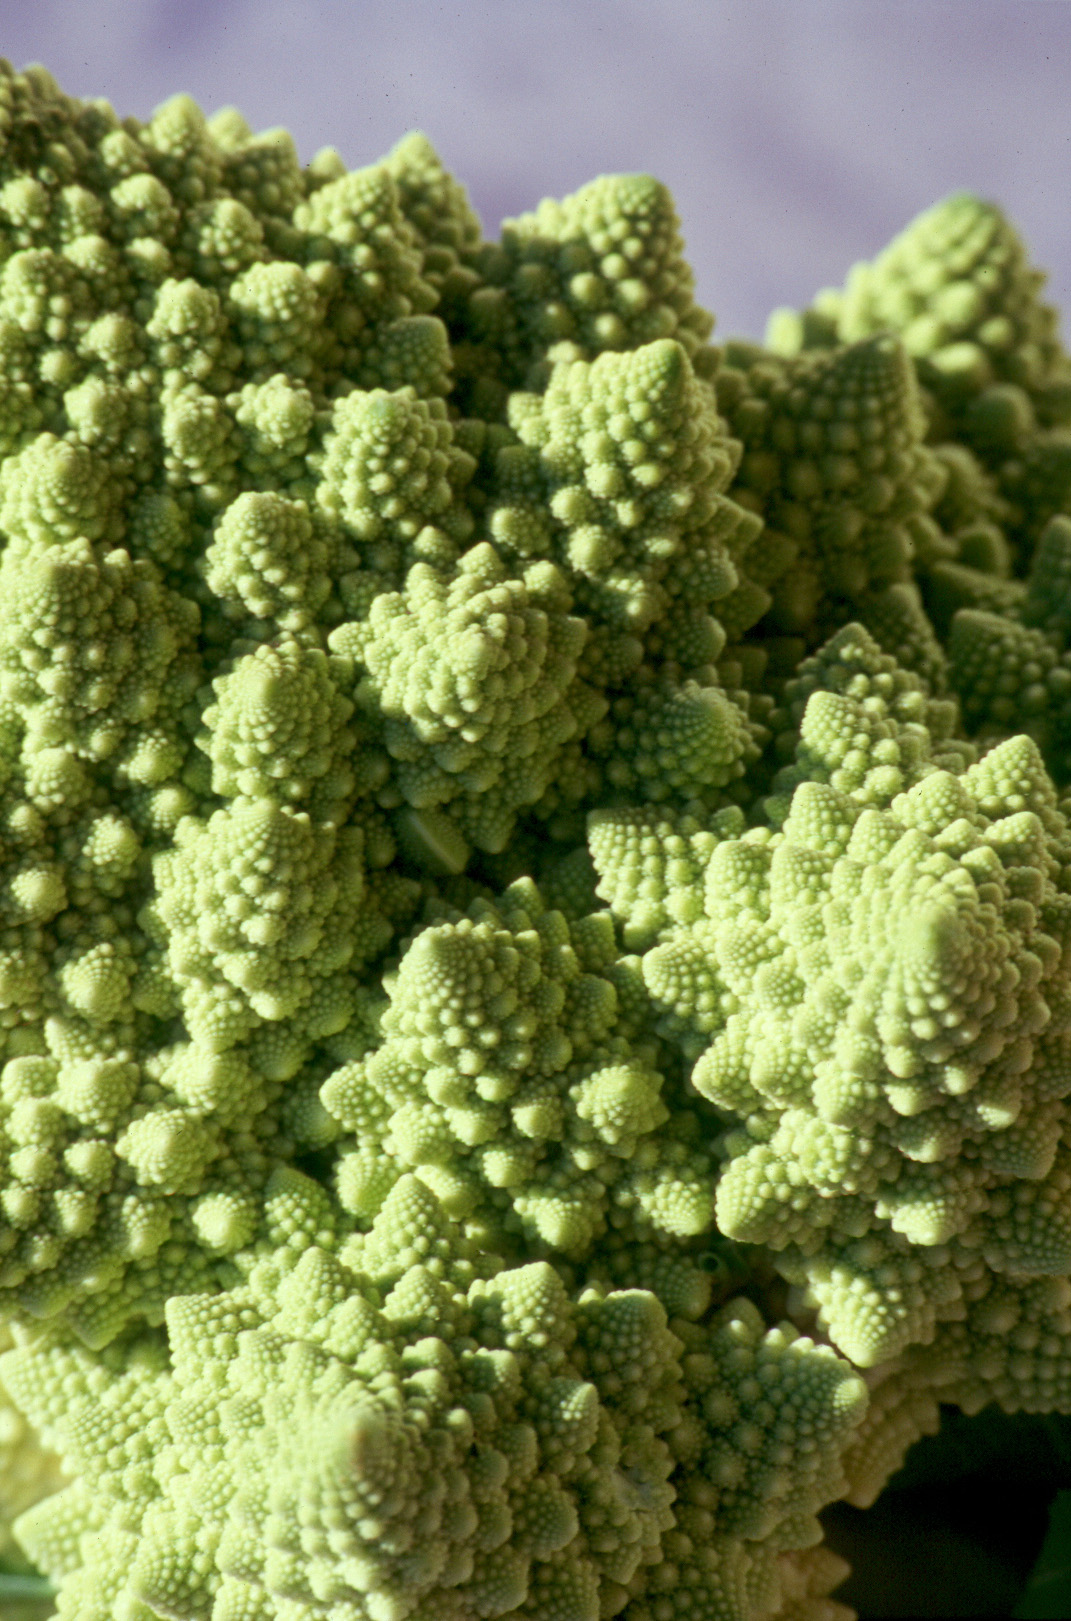
\includegraphics[width=.6\linewidth]{figures/Romanesco}
		\caption{Der Romanesco. Ein natürliches Fraktal.\\\tiny{https://de.wikipedia.org/wiki/Datei:Romanesco.jpg}}
		\label{fig:frac_natur}
	\end{subfigure}%
	\begin{subfigure}{.5\textwidth}
		\centering
		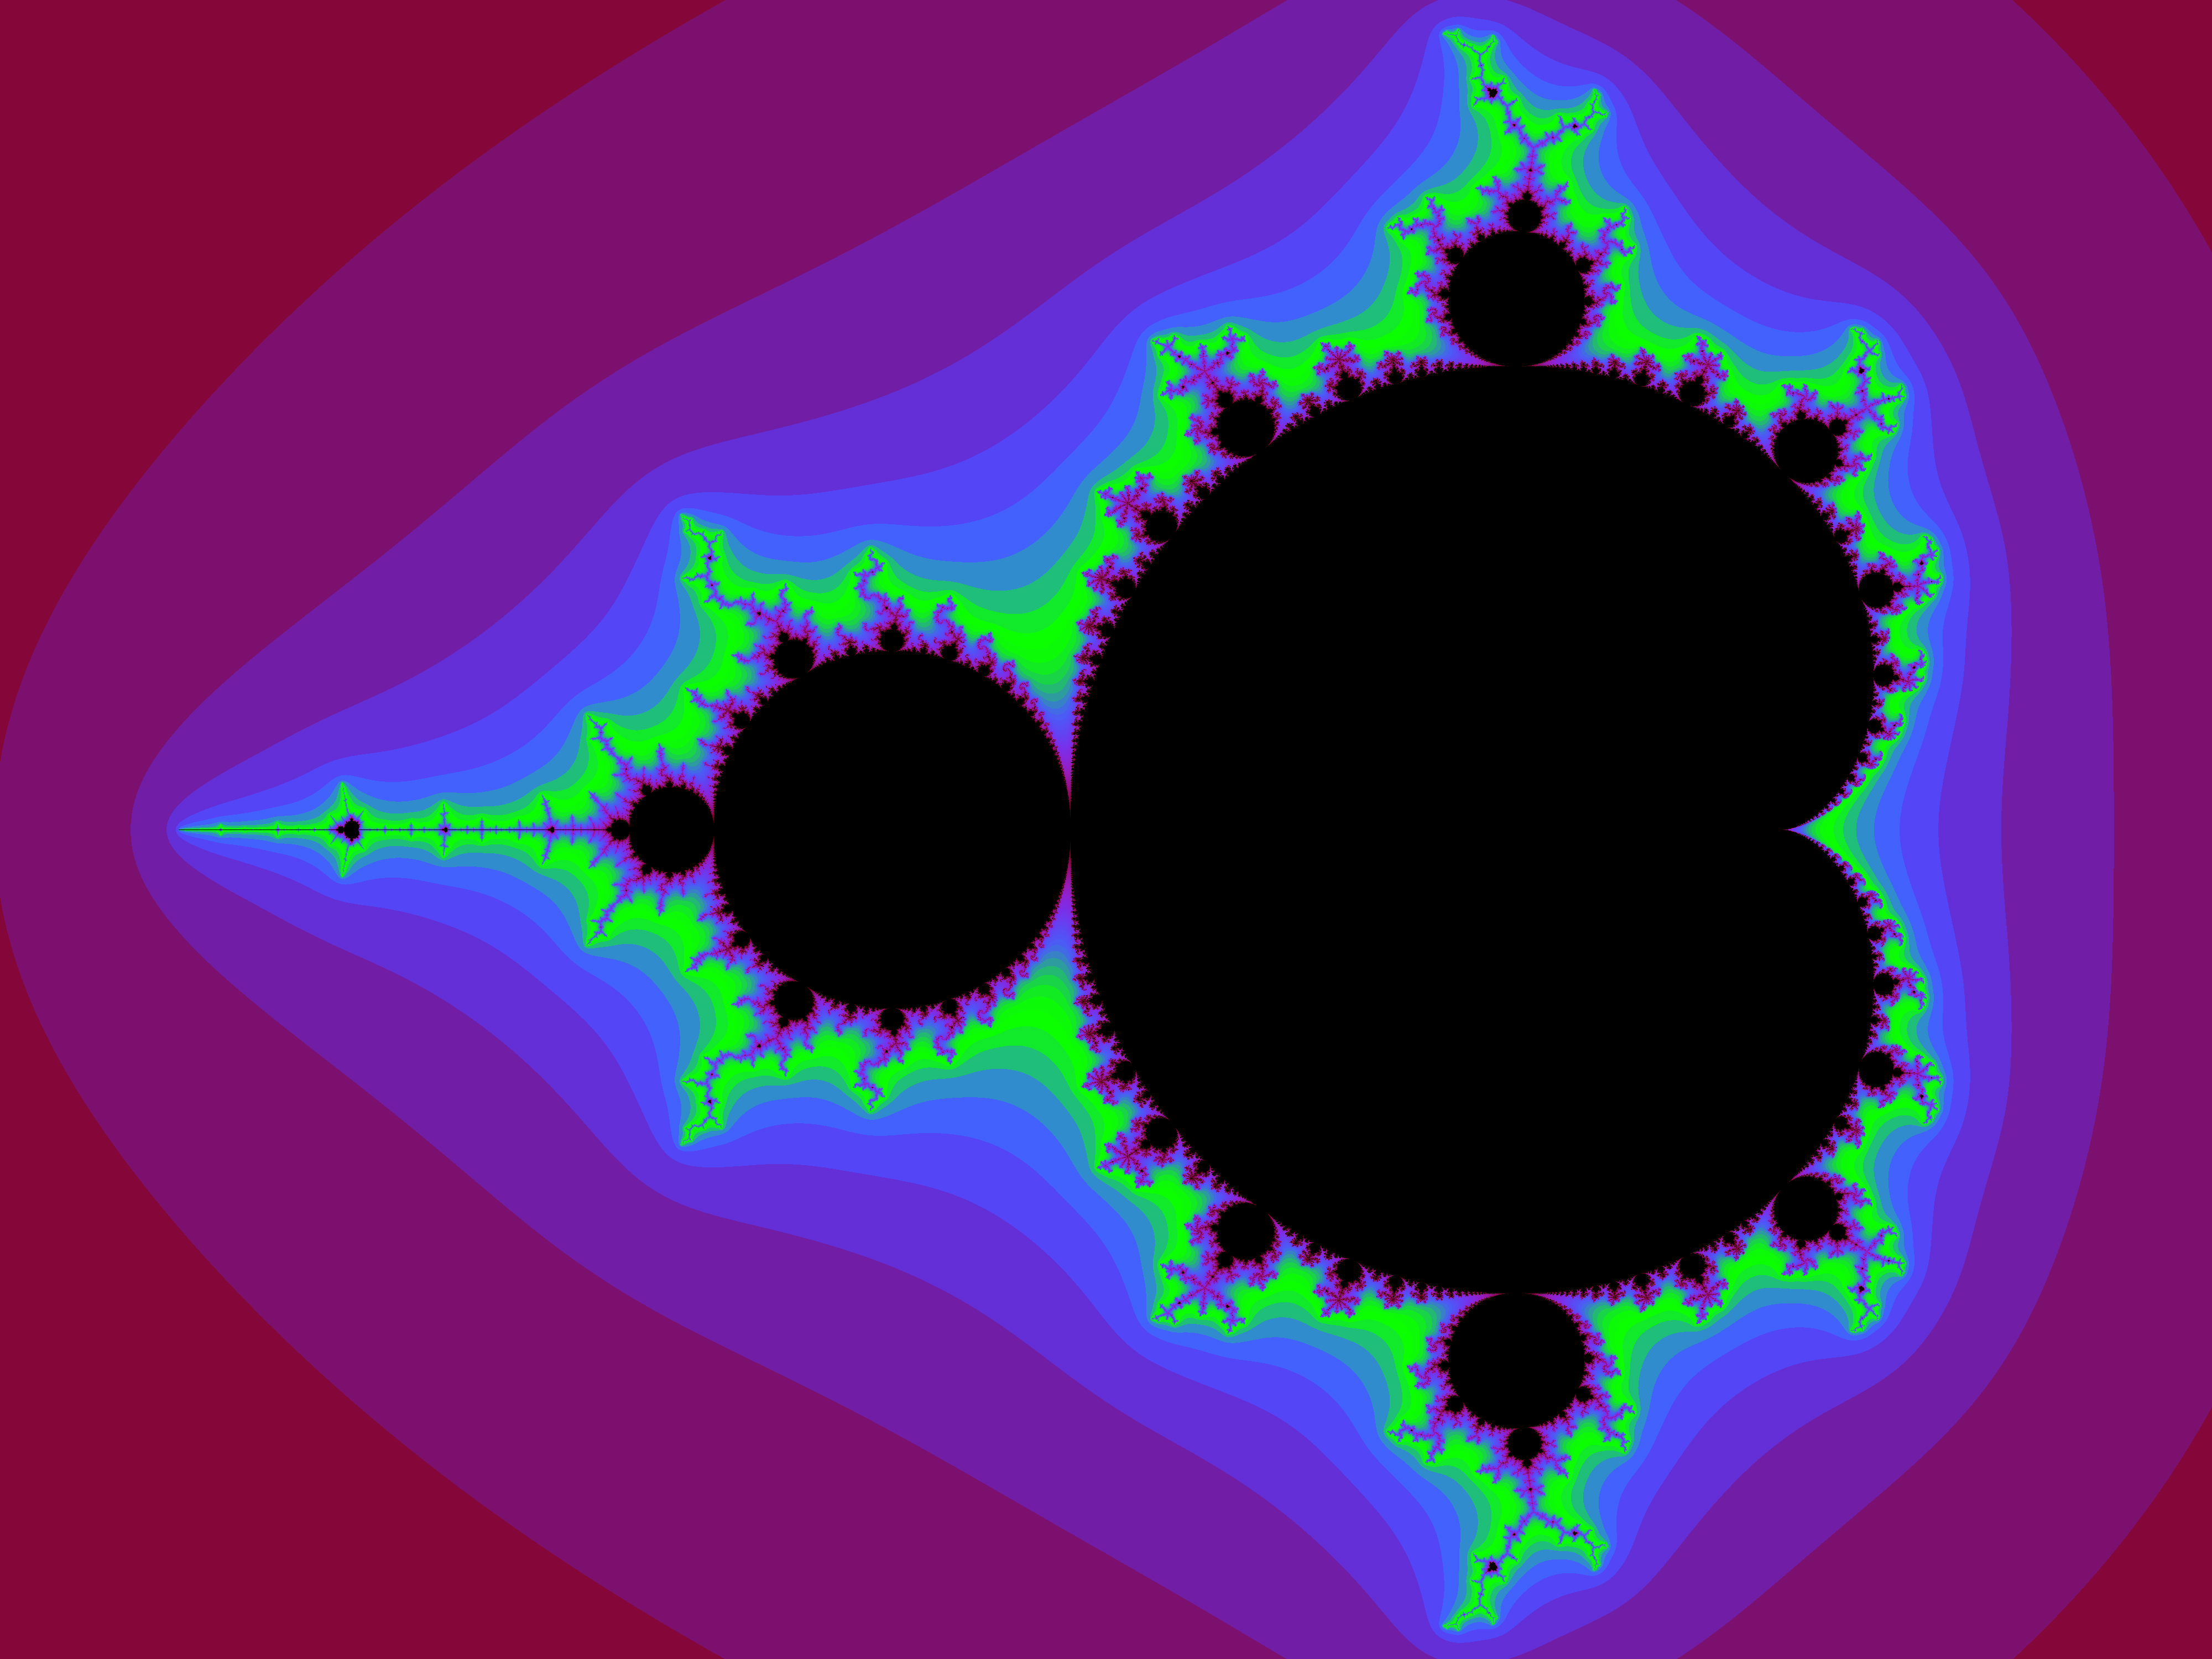
\includegraphics[width=.9\linewidth, angle =90 ]{figures/Mandelbrot}
		\caption{Das Mandelbrot. Ein künstliches Fraktal.\\\tiny{https://de.wikipedia.org/wiki/Datei:Mandelbrot\_\\set\_with\_coloured\_environment.png}}
		\label{fig:frac_math}
	\end{subfigure}%
\end{figure}

\subsection{Newton-Fraktale}
Diese Fraktale erscheinen, wenn man das Newton-Verfahren für Auffinden der Nullstellen der nichtlinearen Gleichungen auf der komplexen Ebene einsetzt. 
Die komplexe Zahlen werden verwendet, um ein 2D Bild zu bekommen.
Realer Betrag der Zahl wird als die x-Koordinate benutzt und imaginärer Betrag - als die y-Koordinate.
Dann wählt man den Bereich und die Auflösung des gesuchten Bildes (zum Beispiel ein Quadrat mit $x\in\{-1;+1\}$ und $y\in\{-1;+1\}$ mit der Auflösung $100x100$) und bemalt es.
Genauer gesagt, benutzt man die Position jedes Pixels des Bildes als der Startwert für das Newton-Verfahren und schaut gegen welche Nullstelle es konvergiert.\\
Zum Beispiel nehmen wir die Funktion $f(x) = x^3 -1$. 
Diese Funktion hat drei Lösungen auf der komplexen Ebene: $1$, $-\sqrt[3]{-1}$ und $(-1)^{2/3}$. 
Die Näherungswerte im Koordinatenform sind $(1, 0)$, $(-0.5, 0.866)$ und $(-0.5, -0.866)$. 
Die Punkte des Bildes, die sich durch das Newton-Verfahren zu entsprechenden Nullstellen annähern, werden entsprechend mit rot, blau und grün gefärbt.
Das Fraktal auf dem Bild~\ref{fig:output3_0} repräsentiert die gewählte Umgebung.
Die Ursachen der bemerkenswerten Mischung werden in der Sektion~\ref{sec:analy} erläutert.
\begin{figure}[ht]   
	\centering
	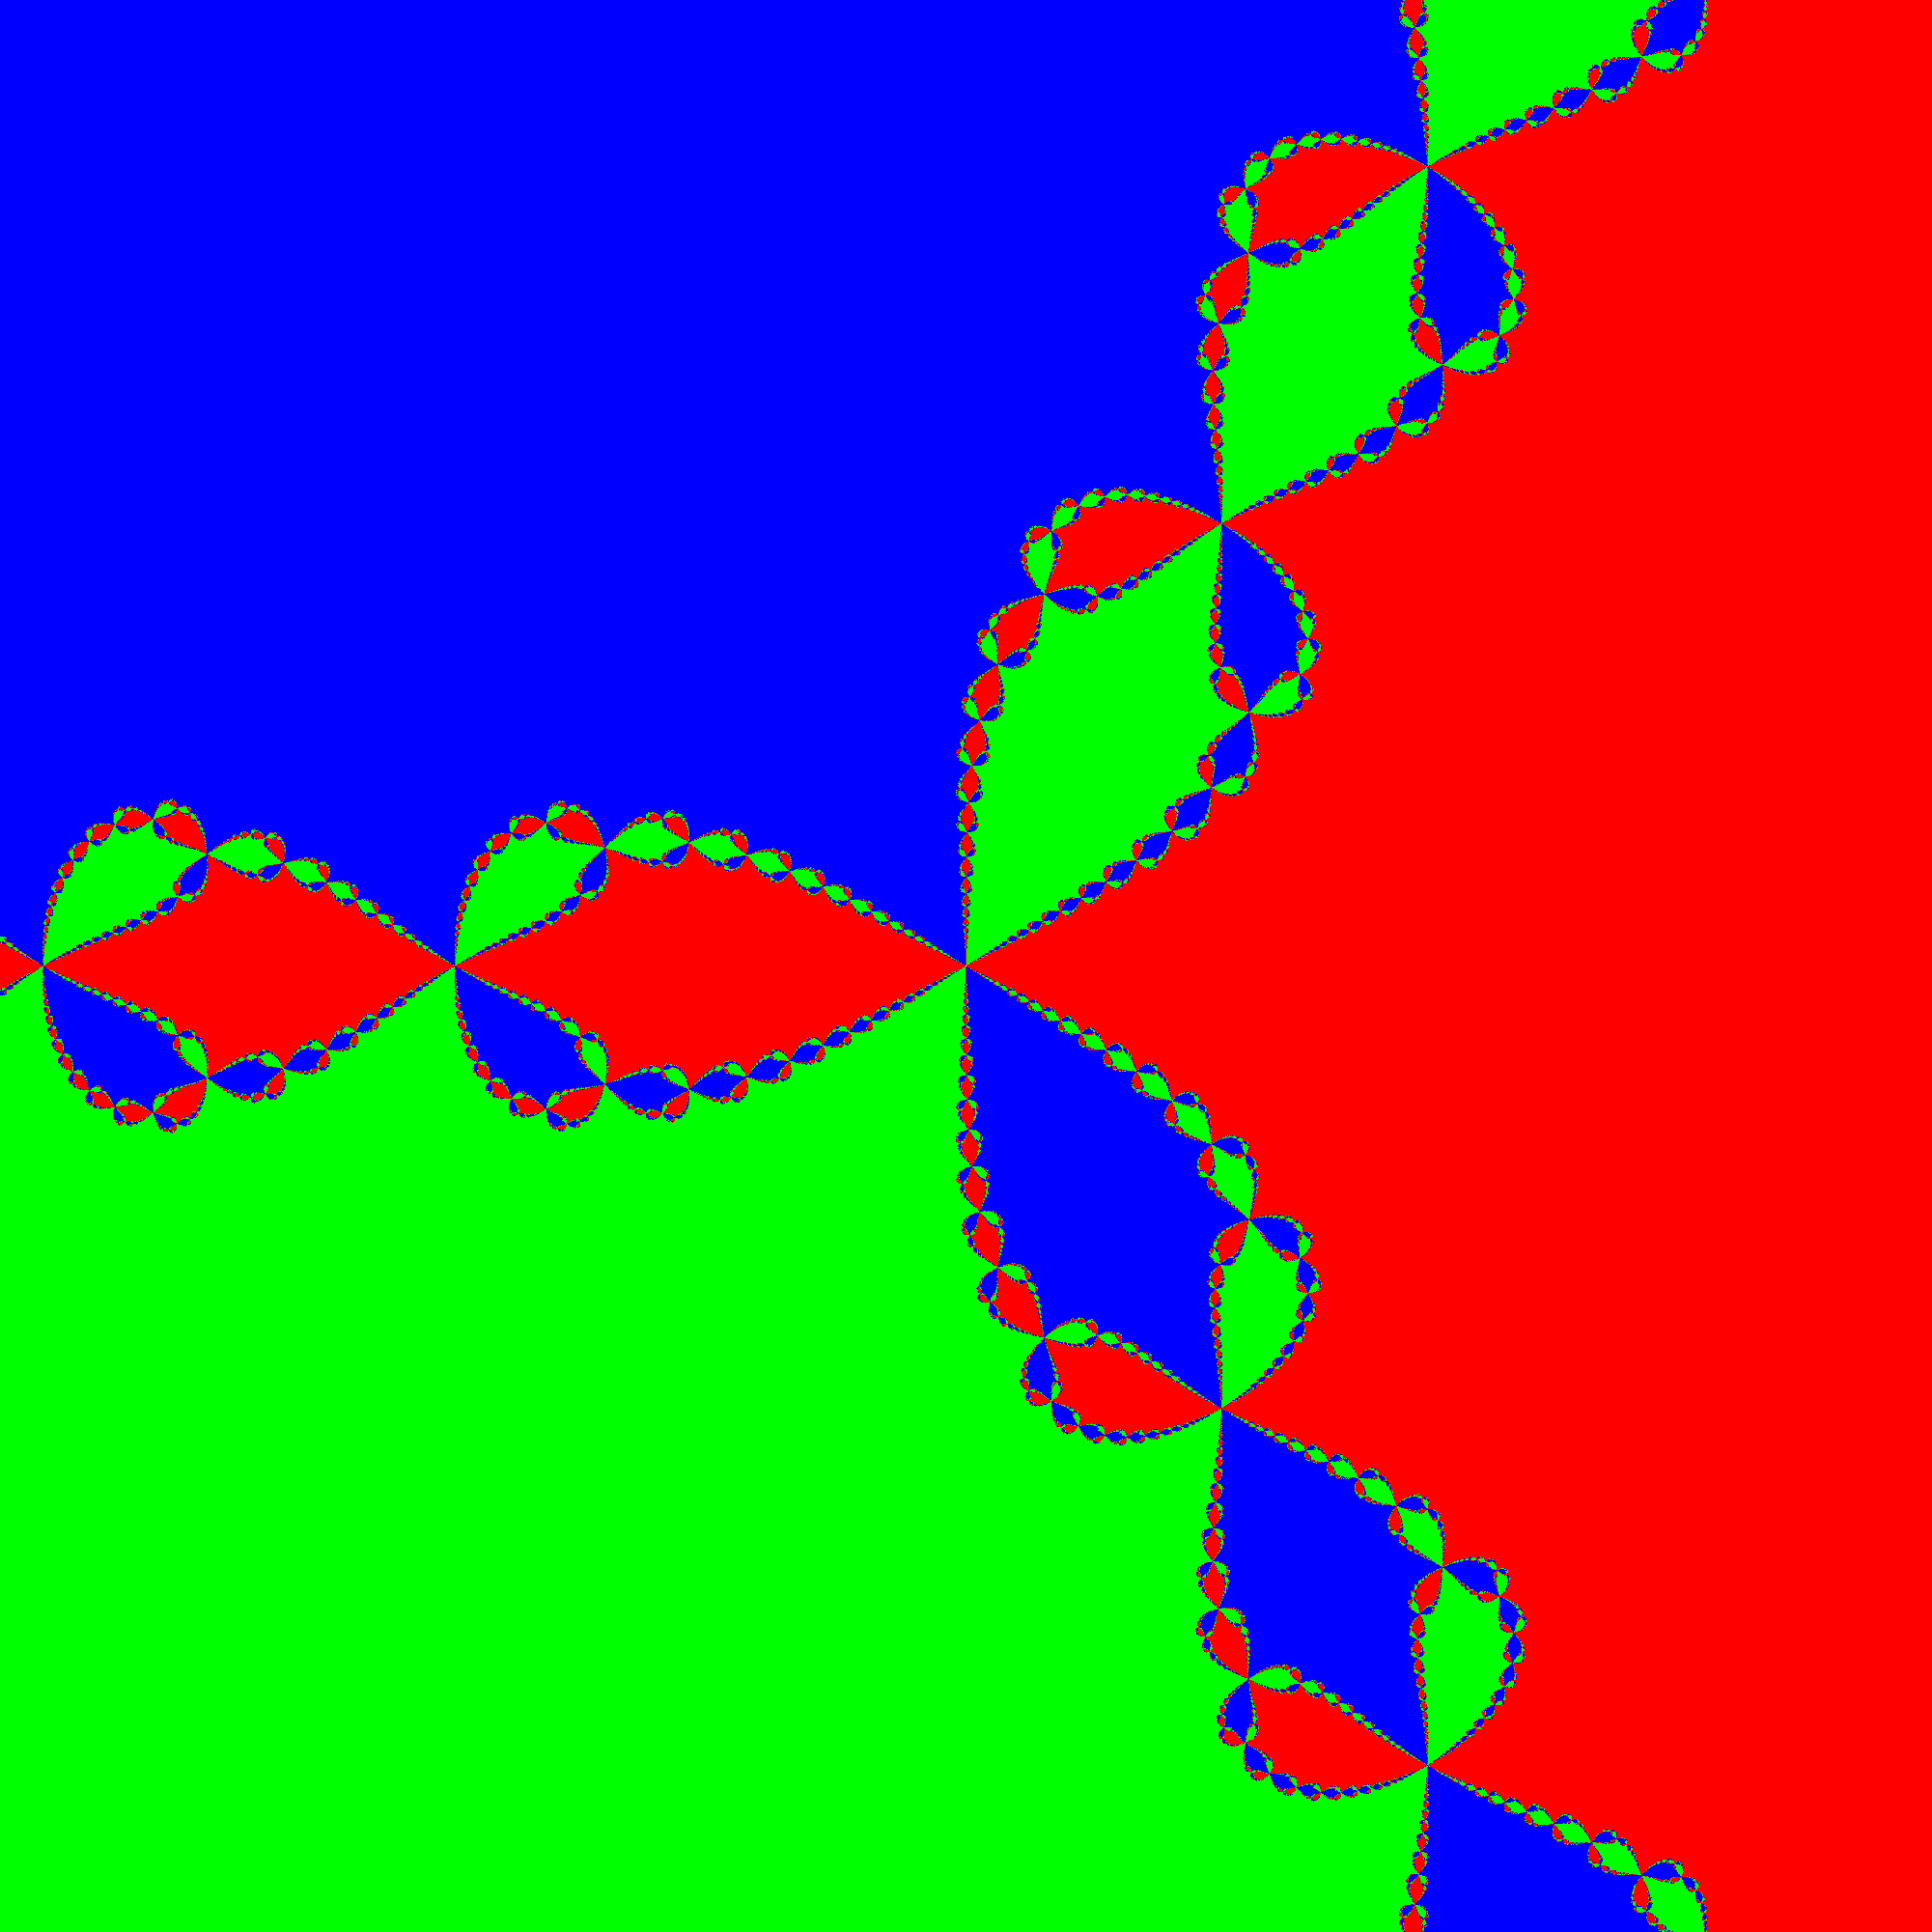
\includegraphics[width=.5\linewidth]{figures/output3_0}
	\caption{Newton-Fraktal für $f(x)=x^3-1$ }
	\label{fig:output3_0}
\end{figure}

\section{Visualisierung}\label{sec:vis}
In diesem Abschnitt wird ein Programm entwickelt, das Bilder mit der Newton-Fraktale generiert.
Außerdem wird ein Beispiel vorgestellt, wie man Animationen erzeugen kann.

\subsection{Bildgenerierung}\label{subs:vis:bild}
Hier wird ein Programm beschrieben, die Newton-Fraktale visualisiert.
Als Programmiersprache wurde Java gewählt.

\subsubsection{Bibliotheken}
Zusätzlich zur allgemeinen Java-Bibliothek wurde noch\\ \verb|javax.imageio.ImageIO| verwendet.
Das ist eine öffentliche Bibliothek für die Arbeit mit Bildern, die unter anderem für das .$png$ Format geeignet ist.
Das PNG (Portable Network Graphics) Format passt für unsere Ziele ideal wegen kleines Gewichtes und keines Qualitätsverlustes der Dateien.

\subsubsection{Bild}
Mit Hilfe von \verb|javax.imageio.ImageIO| kann man die .$png$ Bilder sehr einfach erzeugen. 
Ein Beispiel ist in der Auflistung~\ref{lst:png}.
\begin{lstlisting}[float,caption=Ein Beispiel für die PNG Generierung, label=lst:png,captionpos=b]
BufferedImage bi = new BufferedImage(width, height, TYPE_INT_ARGB) ;
ImageIO.write(bi, "png", outputfilename);
\end{lstlisting}
Um den Bildinhalt einzusetzen, benutzt man den \verb|bi.setRGB(x, y, Color);| Befehl.\\
Natürlich muss man einen bestimmten Bereich des Fraktals wählen, um es zu zeichnen. 
Bei dem Programm wählt man den Startpunkt durch $X$ und $Y$ Koordinatenwerte, die Bildschirmgröße $size$ und die Auflösung $resolution$. 

\subsubsection{Komplexe Zahlen}
Für die Bearbeitung der komplexen Zahlen ist eine neue Klasse implementiert, die die Arbeit mit komplexen Zahlen erleichtert. 
So kann man komplexe Zahlen addieren, subtrahieren, multiplizieren, dividieren und potenzieren.

\subsubsection{Newton-Verfahren}
Um das Newton-Verfahren zu benutzen, muss man manuell die Ableitung berechnen, die iterative Newton-Funktion ausfinden und sie im Programmkode umwandeln.
Außerdem assoziiert man mit jeder Wurzel eine Farbe, um später das Bild zu zeichnen.
Als Beispiel nehmen wir die Funktion $f(z) = z^3 - 2z + 2$.
Die entsprechende Ableitung hat die Form $f'(z) = 3z^2 - 2$ und die iterative Funktion des Newton-Verfahrens $z_{n+1} = \frac{2z_n^3 - 2}{3z_n^2 - 2}$.
Und hier steht der Programmkode für die iterative Funktion.
\begin{lstlisting}
devide(mult(pow(X,3),2).add(-2),mult(pow(X,2),3).add(-2));
\end{lstlisting}
Die Funktion wird iterativ für jedes Pixel des Bildes verwendet, um die Farbe zu berechnen.
Natürlich muss man nach jedem Schritt prüfen, ob die maximale Anzahl der Schritte $N$ nicht überschritten ist und ob der Punkt schon die Wurzel ist. 
Das heißt, dass es für jeden gefundenen Punkt $z_n$ geprüft werden muss, ob $n > N$ oder $f|(z_n)| < \varepsilon$ ist.
Falls einer der beiden Fälle eintritt, bricht man die iterative Berechnung ab.
Im ersten Fall bezeichnet man den Punkt mit der weißen Farbe, im zweiten - mit der Farbe, mit der man die gefundenen Wurzel assoziiert. 

\subsubsection{Lösungen} 
Da man die Farben für unterschiedliche Wurzeln manuell wählen will, muss man alle Wurzeln mit assoziierten Farben in den Programmkode eintragen. 
Ein Beispiel für die Funktion $z^3 - 1$ findet man in der Auflistung~\ref{lst:punkt}. 
Jede Wurzel wird durch zwei Zahlen festgestellt, die reale und imaginäre Parts abbilden.
Letzte drei Argumente definieren die Farbe der Wurzel im RGB Format.
\begin{lstlisting}[caption=Wurzeln mit Farben für $z^3 - 1$, label=lst:punkt,captionpos=b]
\\Position X, Position Y, rot, gruen, blau
points.add(new point(   1,     0,255,  0,0)); 
points.add(new point(-0.5, 0.866,  0,255,0));
points.add(new point(-0.5,-0.866,  0,  0,255));
\end{lstlisting}

\subsubsection{Helligkeit}
Für bessere Informationswiedergabe darf man optional die Schatten einschalten.
Dann je mehr Schritte des Newton-Verfahrens nötig sind, desto dunkler das Pixel wird.  

\subsubsection{Programmkode}
Den vollständigen Programmkode kann man unter~\cite{source} finden.

\subsection{Animation}\label{subs:vis:anime}
Einer der einfachsten Wege für die Animationserzeugung wurde gewählt. 
Das Programm wurde so geändert, damit $size$ und $outputfilename$ variabel werden. 
Dann wird eine Reihenfolge der Bildern im Zyklus generiert, so dass das neue Bild die Annäherung des Alten wird.
Die Animation wird aus dieser Reihenfolge der Bilder mit Hilfe des~\cite{animegen} generiert und als eine .$gif$ Datei vorgestellt.

\section{Analyse}\label{sec:analy}
Manche Newton-Fraktale werden vorgestellt und analysiert.

\subsection{Newton-Fraktale der Gleichung $z^3 - 1 = 0$}
Wie oben schon gesagt wurde, hat diese Gleichung drei Lösungen auf der komplexen Ebene: $+1$, $-\sqrt[3]{-1}$ und $(-1)^{2/3}$.
Die iterative Funktion hat die folgende Form:
\[
x_{n+1} = \frac{x_n^3+1}{3 x_n^2}
\] 
Entsprechendes Newton-Fraktal ist auf dem Bild~\ref{fig:output3_0} visualisiert. 
Wenn man versucht, die Grenze zwischen zwei Zonen zu annähern, sieht man, dass dort immer eine dritte Zone vorkommt. 
Das wiederholt sich rekursiv bei Annäherung.
In anderen Worten, wenn man einen Punkt $z_0$, der gegen $+1$ konvergiert, und einen Punkt $z_1$, der gegen  $-\sqrt[3]{-1}$ konvergiert, wählt, dann existiert zwischen $z_0$ und $z_1$ immer einer dritter Punkt $z_2$, der noch näher zu $z_0$ als $z_1$ liegt und gegen $(-1)^{2/3}$ konvergiert. \\
Wichtigste Frage ist: warum sehen die Zonen nicht wie die einfachen 120-Grad-Sektoren aus?
Anfang letztes Jahrhunderts gelang es zwei französischen Mathematiker Gaston Julia und Pierre Fatou zu zeigen, dass die Grenzpunkte eines Einzugsgebiets die Grenzpunkte aller Einzugsgebiete sind. 
Folglich können Iterationen mit mehr als zwei Einzugsgebieten keine einfach zusammenhängenden Liniensegmente als Gebietsgrenzen in 2D haben. 
Solche Grenzen müssen zwangsläufig fraktaler Natur sein, bestehend aus vollständig separaten Punktmengen - sozusagen eine unendlich feine Staubwolke aus nichtabzählbar vielen Staubpartikelchen.~\cite{frak_cha}\\
Machen wir uns damit ein bisschen vertraut, indem wir den Ursprung (den Punkt $0, 0$) anschauen.
Logischerweise soll der Ursprung zwischen allen Zonen liegen.
Der Punkt selbst konvergiert überhaupt nicht, da die Einsetzung $z=0$ in die iterative Formel zur Division durch Null folgt. 
Aber nicht nur der Ursprung besitzt diese Eigenschaften.
Es existieren noch unendlich viele Punkte, die gegen den Ursprung konvergieren und für die auch gilt, dass daneben alle Zonen vorhanden sind.
(Das folgt aus der linearen Natur des Newton-Verfahrens.)
Die Punkte bilden diese interessante Grenze zwischen den Zonen.\\
Zum Beispiel betrachten wir die Punkte (1, 1) und (0.9, 1). 
Die Konvergenz des Punktes (1, 1) wird auf dem Bild~\ref{fig:output_points3} vorgestellt.\\
\begin{figure}[ht]   
	\nocaption
	\begin{subfigure}{.5\textwidth}
		\centering
		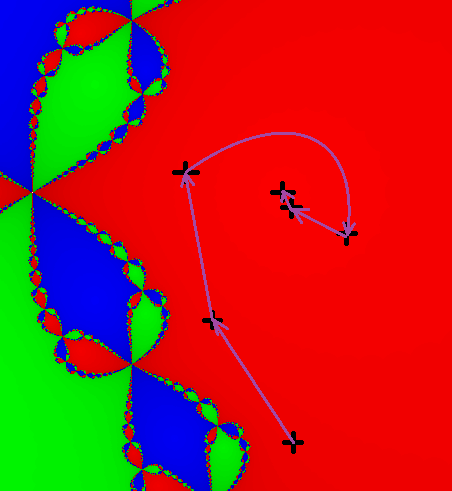
\includegraphics[width=.8\linewidth]{figures/output_points3}
		\captionsetup{width=0.8\textwidth}
		\caption{Die Konvergenz des Punktes (1, 1) für $f(z)=z^3-1$ }
		\label{fig:output_points3}
	\end{subfigure}%
	\begin{subfigure}{.5\textwidth}
		\centering
		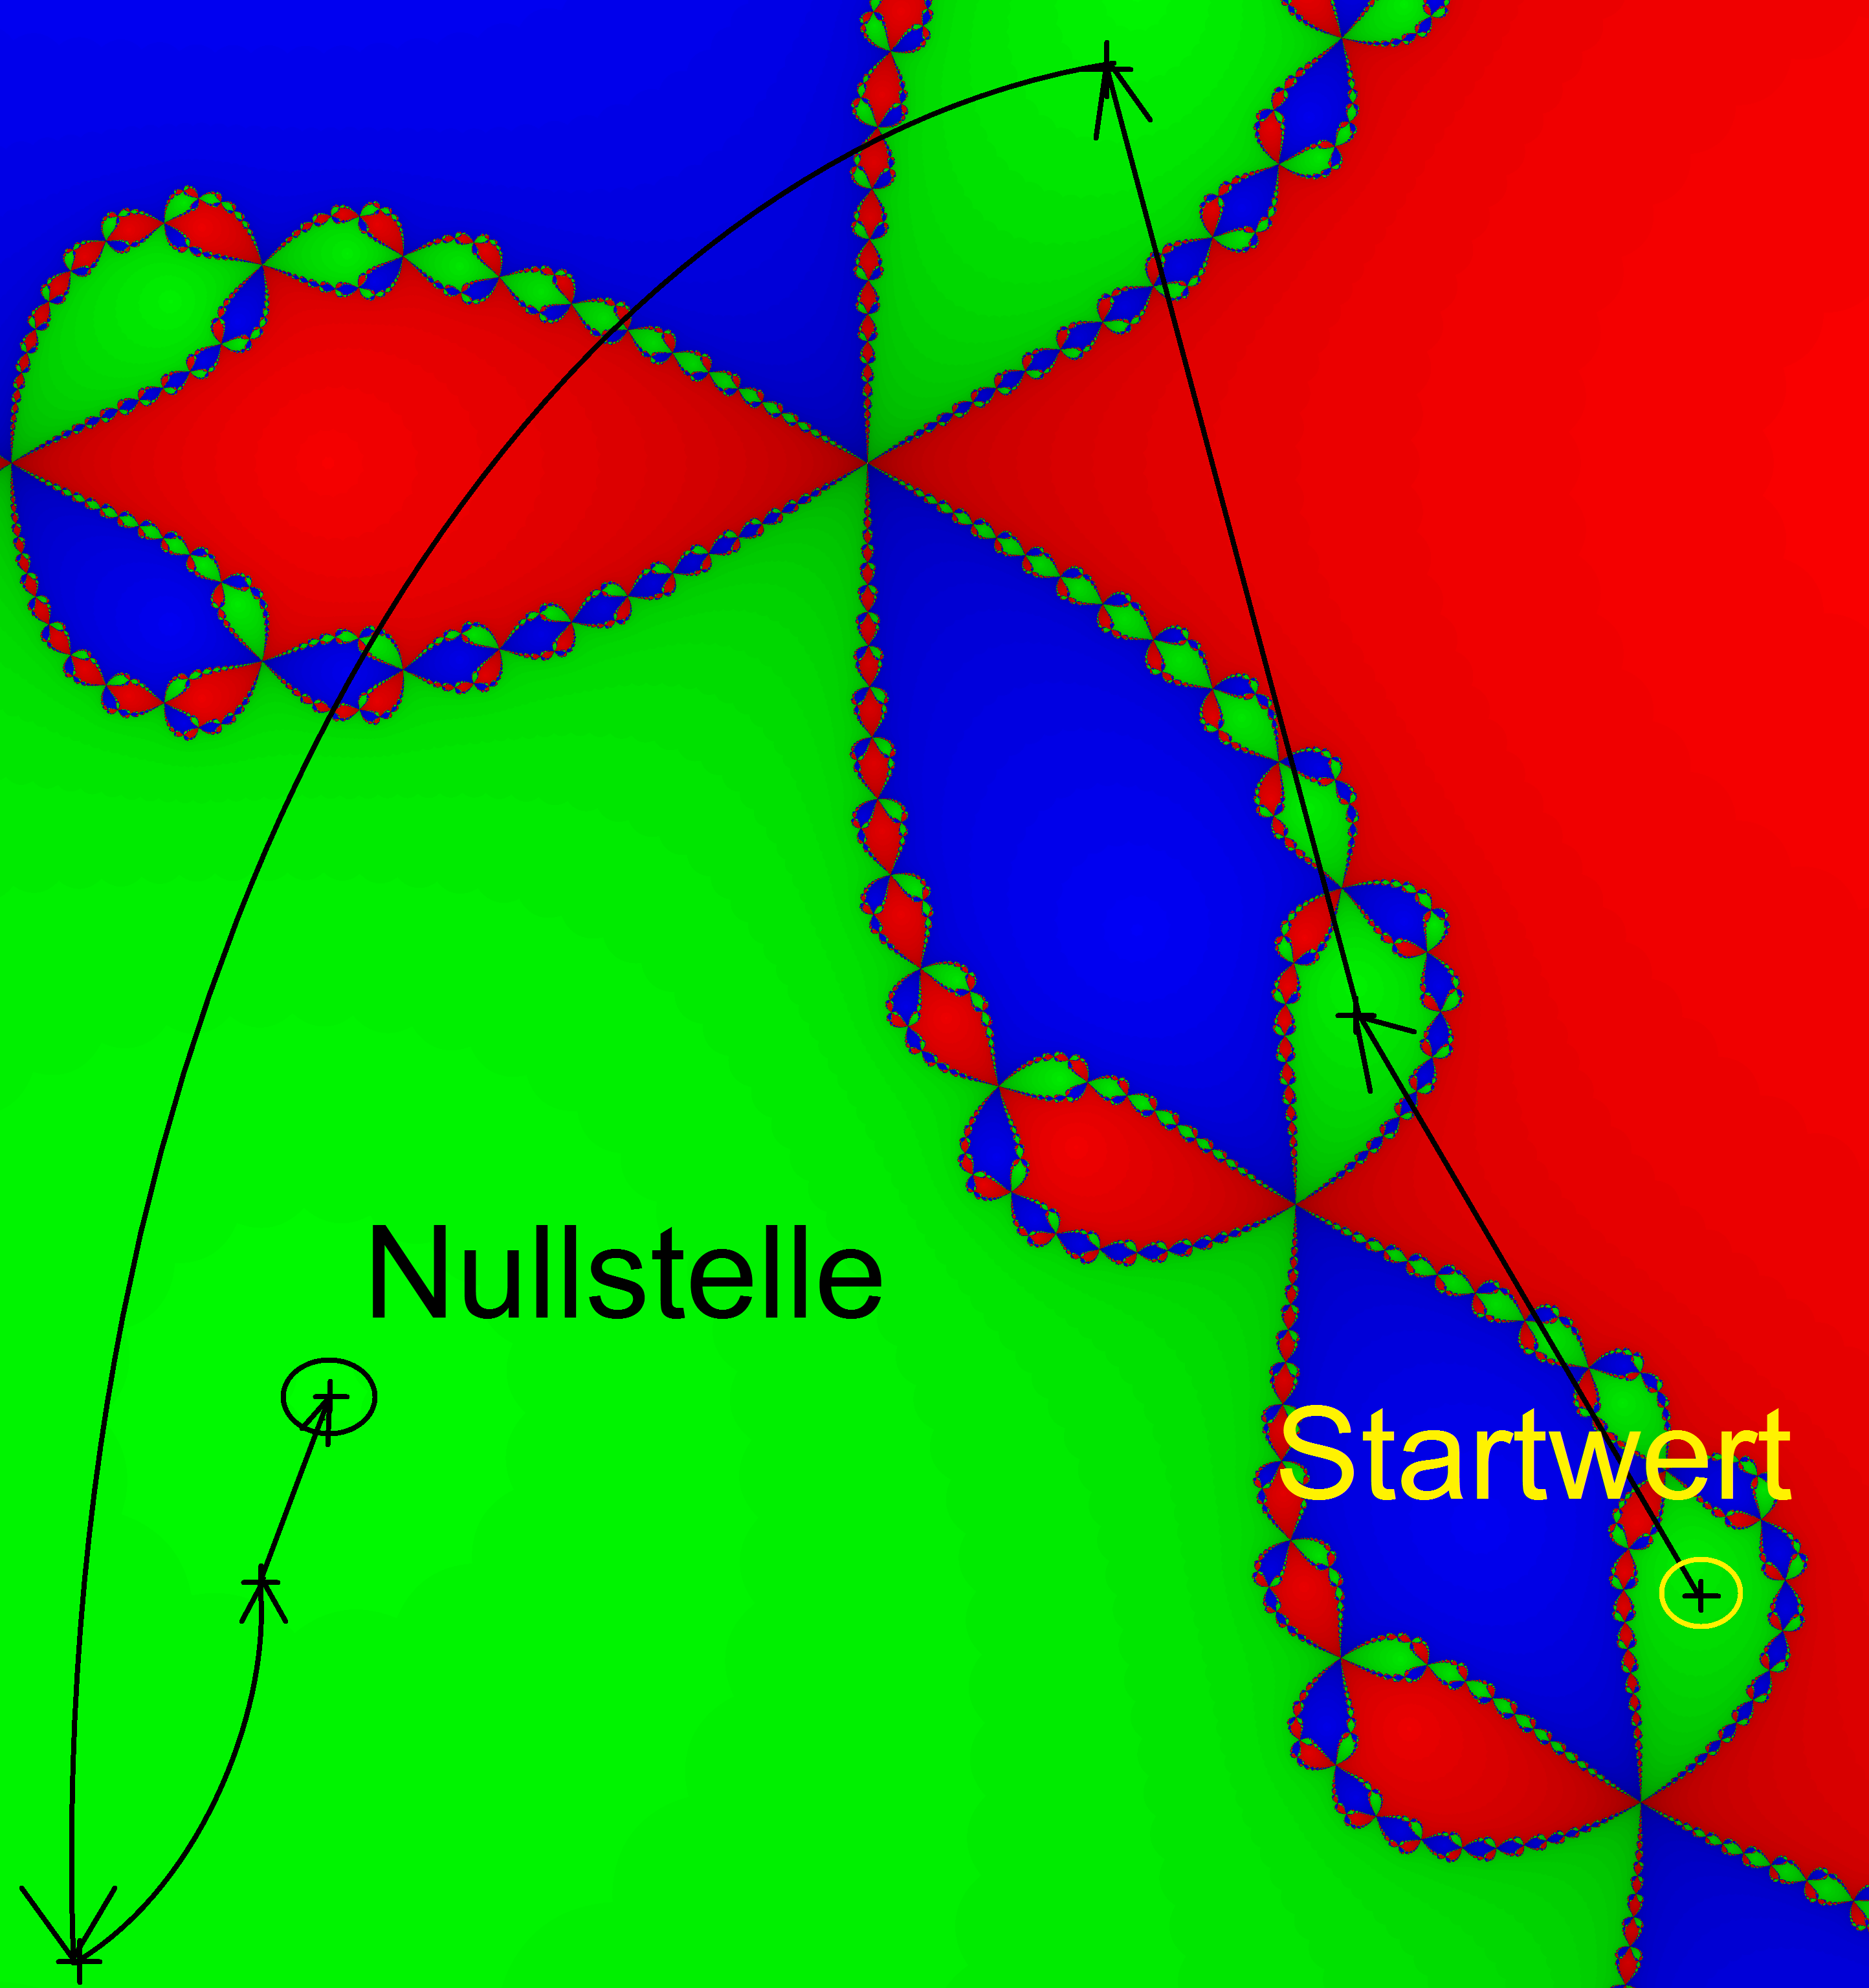
\includegraphics[width=.8\linewidth]{figures/output_points_g3}
		\captionsetup{width=0.8\textwidth}
		\caption{Die Konvergenz des Punktes (0.9, 1) für $f(z)=z^3-1$ }
		\label{fig:output_points_g3}
	\end{subfigure}%
\end{figure}
Der Punkt liegt weit genug von der Grenze und wird eindeutig konvergiert, trotzdem sieht man so einen Sprung, die sehr oft bei Newton-Verfahren eintreten können.\\
Jetzt betrachten wir den Punkt (0.9, 1) auf dem Bild~\ref{fig:output_points_g3}.
Die Konvergenz des Punktes zeigt eindeutig, wie die iterativen Schritte des Newton-Verfahrens funktionieren und wie man zu solchen Bilder kommt. 
Erste zwei iterative Schritte verhalten sich gleich wie bei dem Punkt (1, 1), was die lineare Natur des Newton-Verfahrens bekräftigt. 
Aber dann, neben der Nullstelle, wird es nach grünem Gebiet geworfen.
Die Punkte neben Grenzen bewegen sich zuerst in die Richtung der Nullstelle und springen dann rasant in die passende Zone.\\
Zusätzliches Beispiel wird auf dem Bild~\ref{fig:output3_3} vorgestellt, wo die hellen Bereiche die am schnellsten konvergierenden Punkte bezeichnen.
\begin{figure}[ht]   
	\nocaption
	\begin{subfigure}{.5\textwidth}
	\centering
		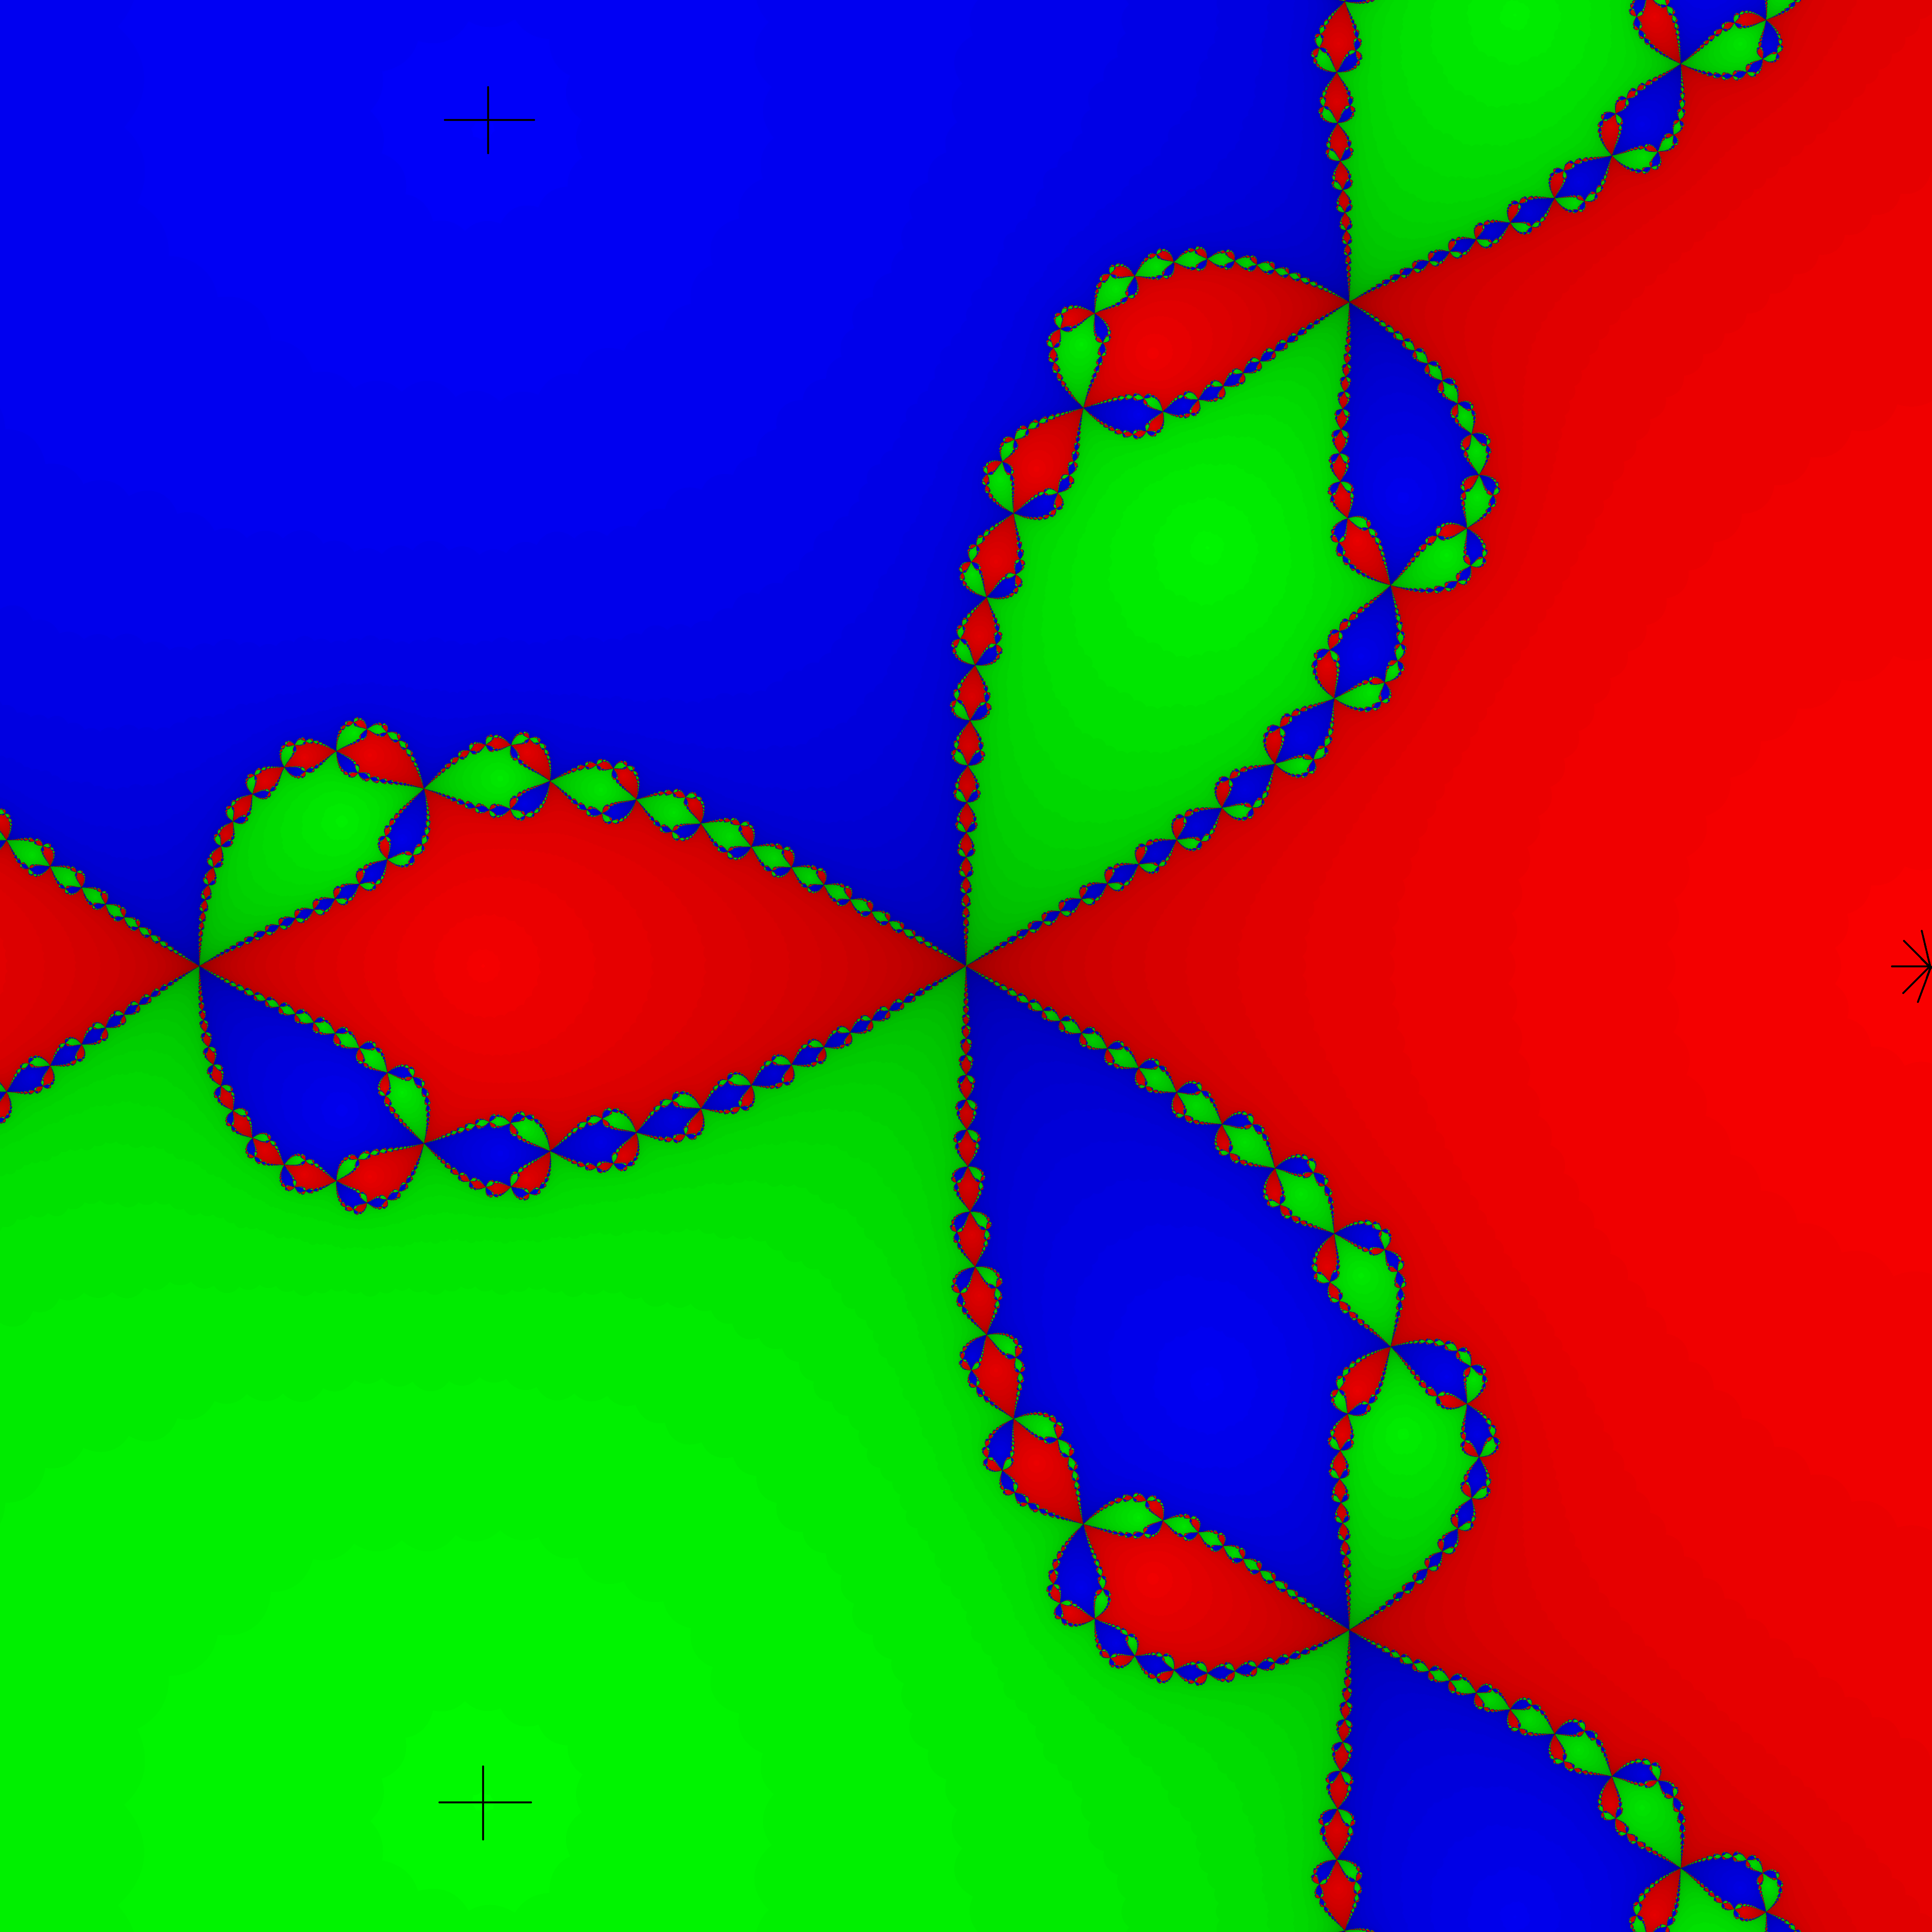
\includegraphics[width=.8\linewidth]{figures/output3_3}
		\captionsetup{width=0.8\textwidth}
		\caption{Die Konvergenzgeschwindigkeit durch die Helligkeit für $f(z)=z^3-1$ }
		\label{fig:output3_3}
	\end{subfigure}%
	\begin{subfigure}{.5\textwidth}
	\centering
		\includegraphics[width=.8\linewidth]{figures/output5_3}
		\captionsetup{width=0.8\textwidth}
		\caption{Das Newton-Fraktal für $f(z)=z^5-1$ }
		\label{fig:output5_3}
	\end{subfigure}%
\end{figure}

\subsection{Newton-Fraktale der Gleichung $z^5 -1 = 0$}
Das Bild~\ref{fig:output5_3} illustriert das entsprechende Newton-Fraktal. 
Der einzige Unterschied liegt in der Anzahl der Zonen und Lösungen.
Die Lösungen sind die Punkte $(1, 0)$, $(-0.809,-0.587)$, $(-0.809,+0.587)$, $(0.309,-0.951)$ und $(0.309,+0.951)$. \\
Wie bei $z^3-1=0$ sind die Grenzpunkte eines Einzugsgebiets die Grenzpunkte aller Einzugsgebiete, was für die fünf Zonen interessanter aussieht.

\subsection{Newton-Fraktale der Gleichung $z^5 + (5+2i)z^3 - 2-i = 0$}
Das entsprechende Newton-Fraktal (das Bild~\ref{fig:output_f7}) besitzt eine interessante Struktur. 
Die Positionen der Lösungen sind die Punkte  $(-0.418,0.640)$, $(-0.4,2.269)$, $(-0.378,-0.645)$, $(0.474,-2.291)$ und $(0.723,+0.026)$.
Der Grund dazu liegt in der Position der Nullstellen.
Der Ursprung, die grüne und die rote Zonen liegen fast auf die Gerade.
Das Gleiche gilt für den Ursprung, die blaue und die hellblaue Zonen.
Unabhängig davon, dass die hellblaue und die grüne Zonen weit weg von dem Ursprung liegen und mit der roten und blauen Zonen abgegrenzt sind, konvergieren manche Punkte neben dem Ursprung gegen das Grün und das Hellblau.
\begin{figure}[ht]   
	\nocaption
	\begin{subfigure}{.5\textwidth}
		\centering
		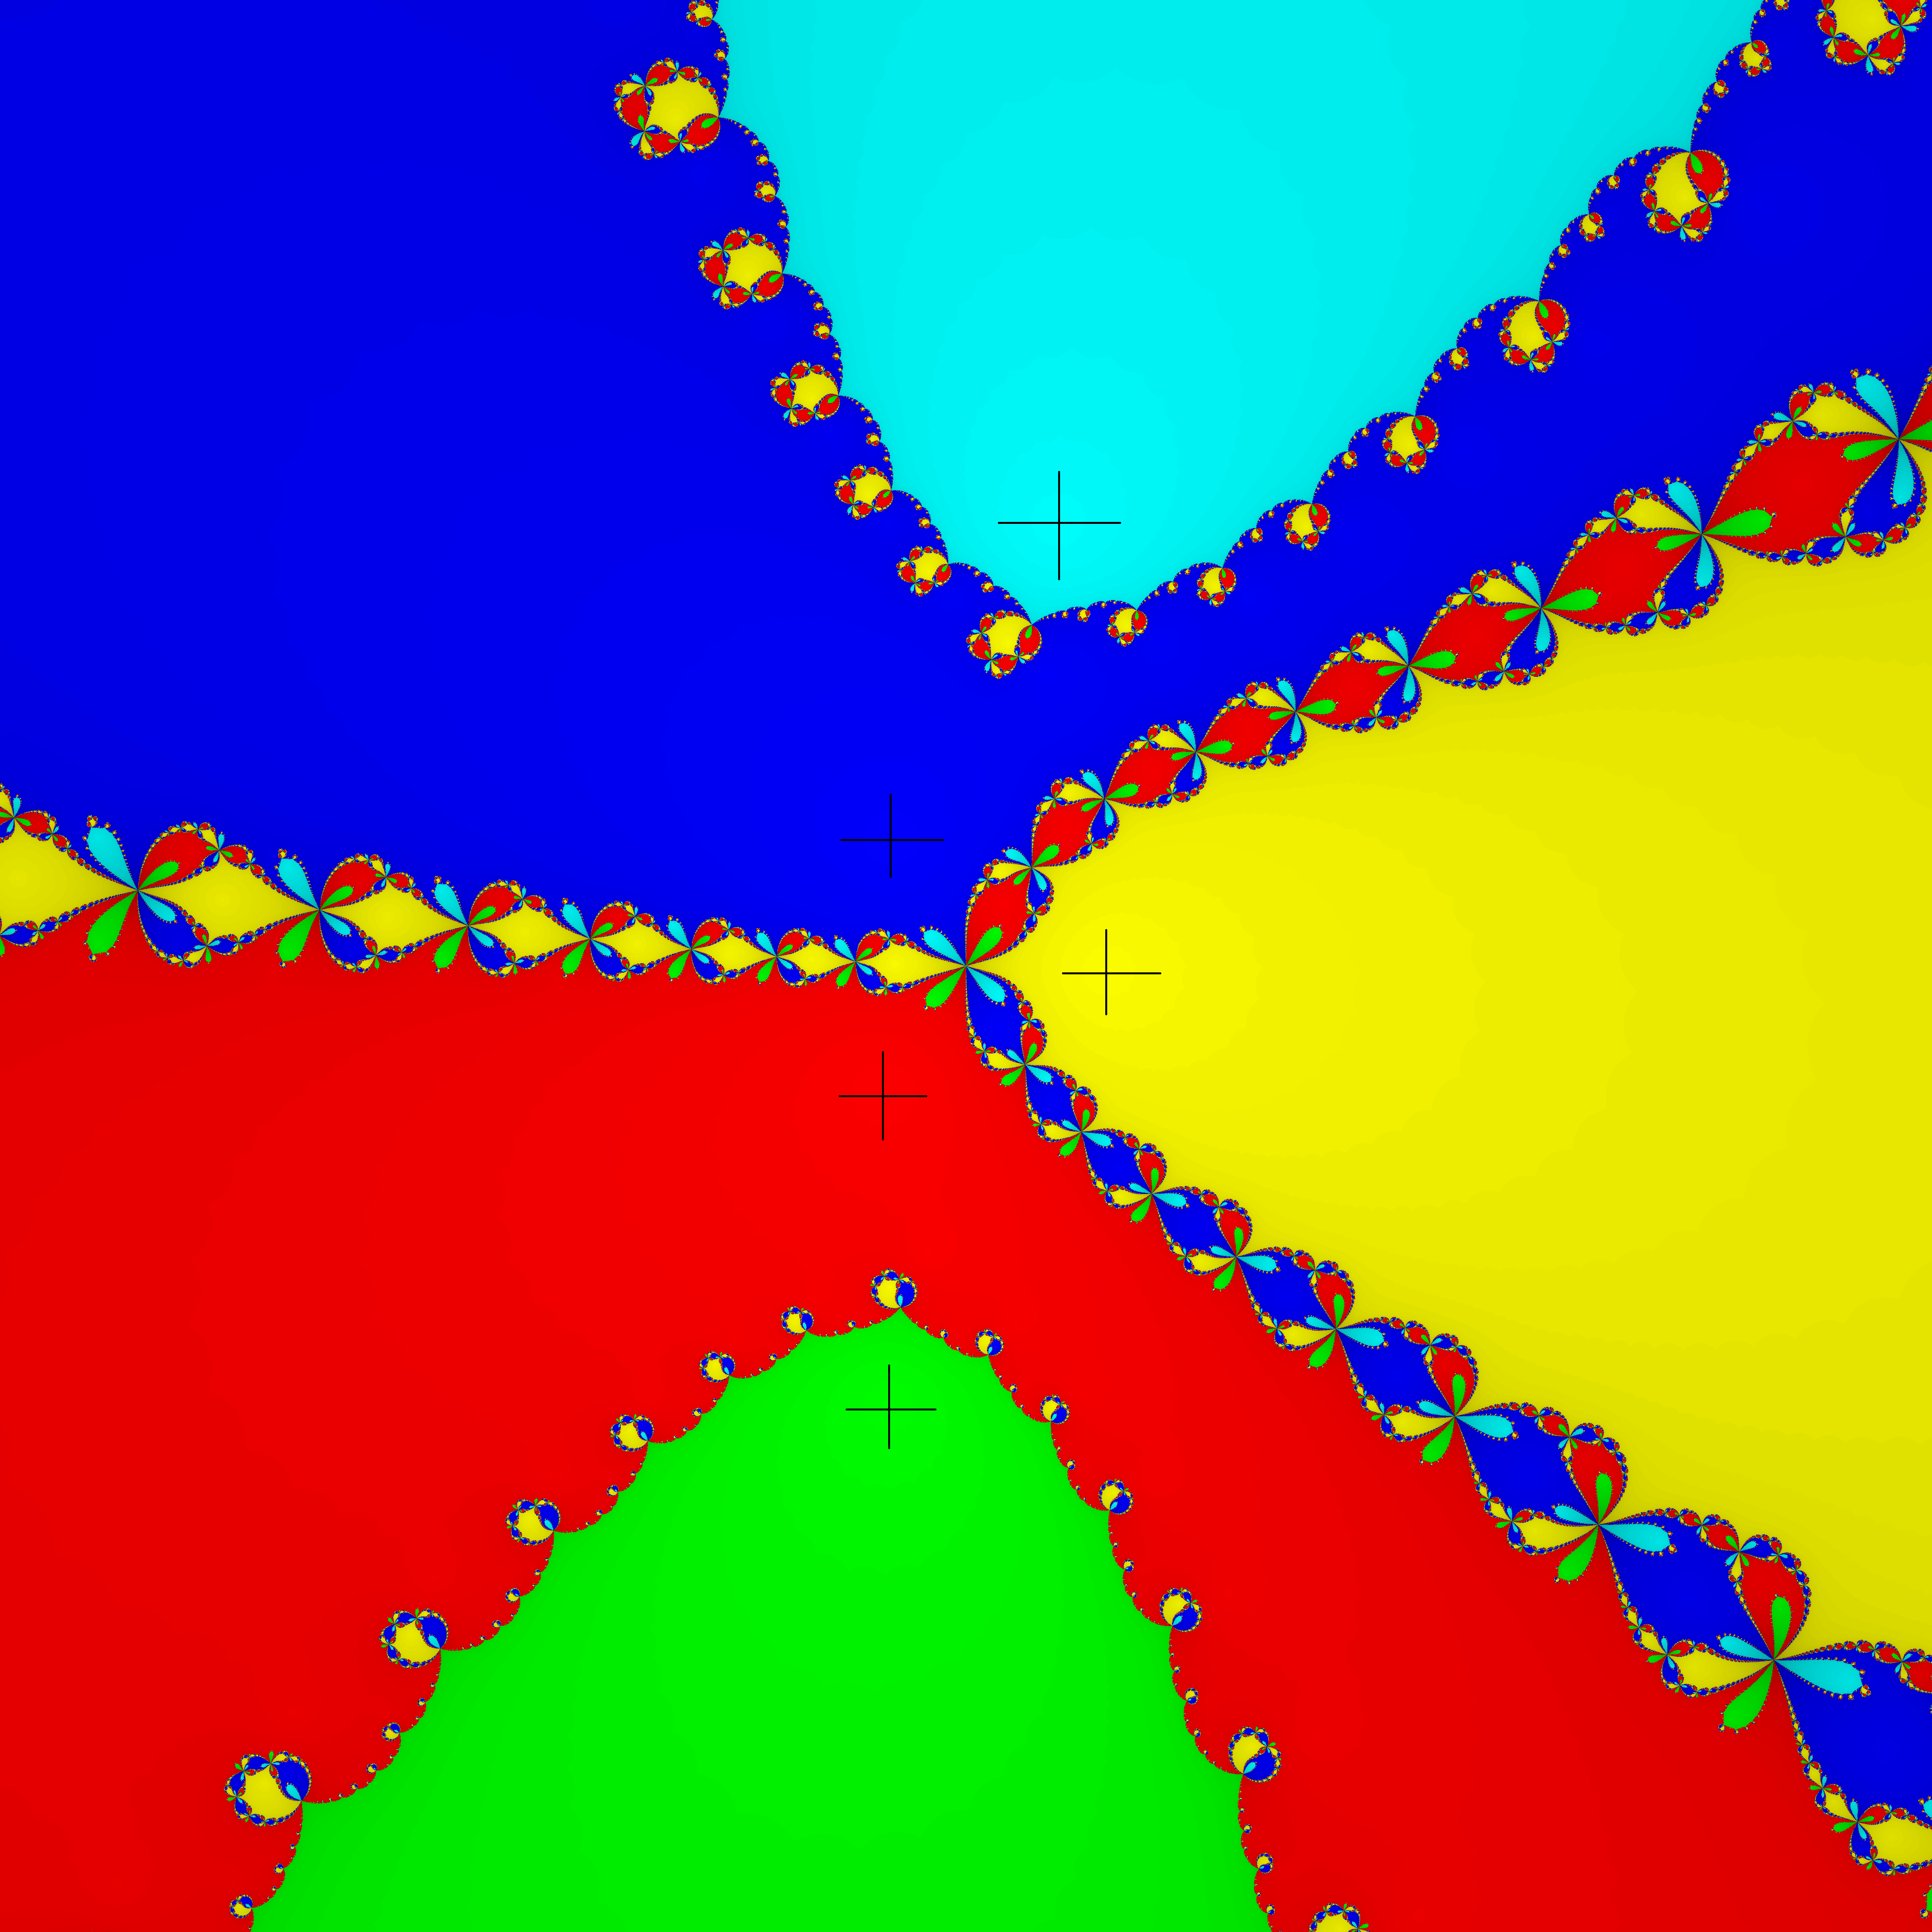
\includegraphics[width=.8\linewidth]{figures/output_f7}
		\captionsetup{width=0.8\textwidth}
		\caption{Das Newton-Fraktal für $f(z)=z^5 + (5+2i)z^3 - 2-i $ }
		\label{fig:output_f7}
	\end{subfigure}%
	\begin{subfigure}{.5\textwidth}
		\centering
		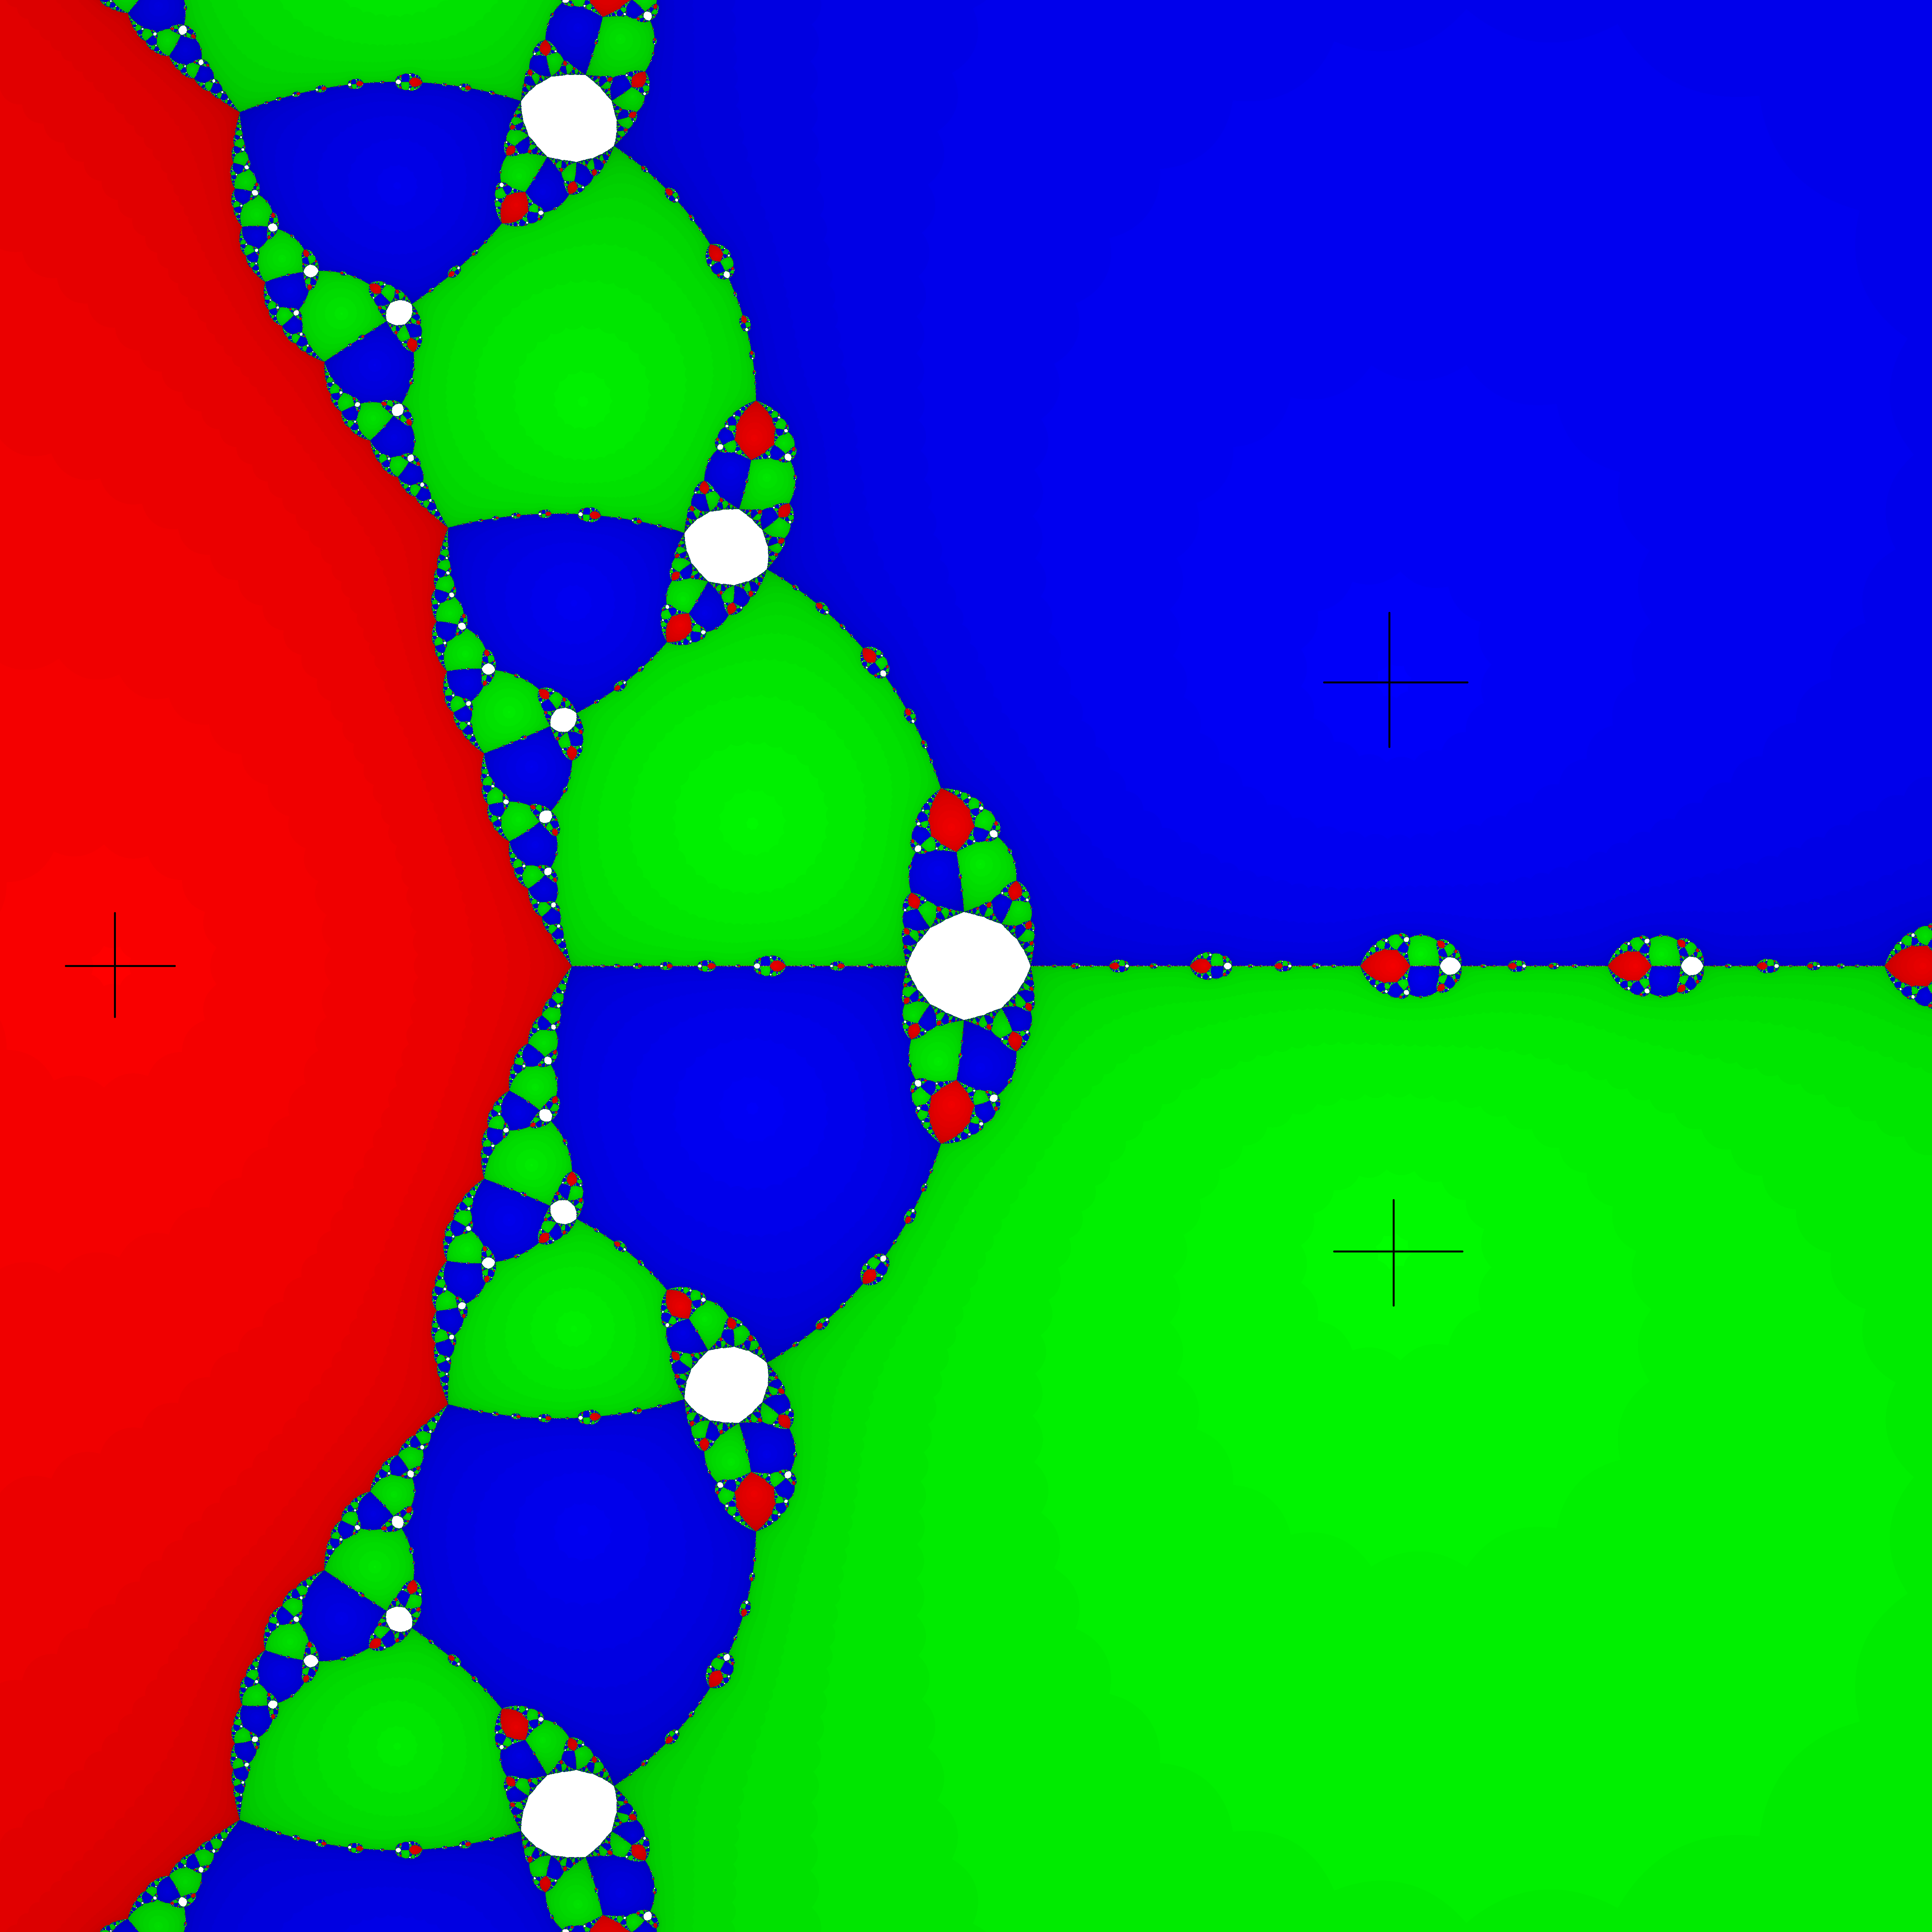
\includegraphics[width=.8\linewidth]{figures/output_f5}
		\captionsetup{width=0.8\textwidth}
		\caption{Das Newton-Fraktal für $f(z)=z^3 - 2z + 2$ }
		\label{fig:output_f5}
	\end{subfigure}%
\end{figure}

\subsection{Newton-Fraktale der Gleichung $z^3 - 2z + 2 = 0$}
Das Bild~\ref{fig:output_f5} illustriert das Newton-Fraktal für diese Funktion.
Die Lösungen sind die Punkte $(-1.769,0)$, $(0.884,0.589)$ und $(0.884,-0.589)$.
Wie man sieht, gibt es hier ziemlich große weiße Bereiche. 
Was passiert dort?
Um diese Frage zu beantworten, müssen wir ein paar Schritte des Newton-Verfahrens manuell ausführen.
Die iterative Funktion hat die folgende Form:
\[
z_{n+1} = \frac{2z_n^3-2}{3z_n^2-2}
\]
Probieren wir den Punkt (0,0) ($z_0 = 0$).
Nach der Einsetzung in die iterative Formel bekommt man $z_1 = 1$.
Sieht noch gut aus, aber was passiert weiter?
Erstaunlicherweise ist $z_2$ wieder gleich $0$.
So springt der Wert zwischen $0$ und $1$, was ein gutes Beispiel dafür ist, warum man die Anzahl der Schritte begrenzen soll.
Aber was passiert neben dem Punkt (0,0), sodass diese weiße Gebiete so groß sind?
Iterieren wir den Punkt (0.1, 0), der ziemlich nah zum Ursprung liegt.
Dann ist $z_0=0.1$; $z_1= 1.014213$ und $z_2= 0.079655$.
Man sieht, dass $z_2$ noch näher zum Ursprung liegt, als $z_0$.
Je mehr iterative Schritte man ausführt, desto näher es zum Ursprung hintritt.
Wenn man versucht, andere Punkte aus der Umgebung dem Ursprung zu iterieren, werden die Punkte, die nah genug liegen, gegen den Ursprung konvergieren.
So werden die weißen Fällen gebildet, die diese Funktion auszeichnen.

\section{Zusammenfassung}
Numerische Lösungen von nichtlinearen Gleichungen durch Approximation sind in der modernen Welt überall gebraucht.
Man berechnet alles von der Wetterprognose und dem Werkzeugmaschinenverhalten bis die Raketensteuerung und die Planetenbahn.
Die approximativen Berechnungen bringen viele unerwartete Probleme und interessante Ereignisse.
Newton-Fraktale sind ein dieser Ereignisse. 
Die Erforschung des Phänomens ist wichtig für unser Verständnis des Newton-Verfahrens. 
Je besser man versteht, wie die numerische Methoden sich verhalten, desto effektiver können sie genutzt werden.\\
Im Rahmen dieser Arbeit wurden theoretische Grundlagen vorgestellt, wichtigste Begriffe erläutert und erklärt.
Dann wurde die Software entwickelt, die manche Newton-Fraktale visualisiert.
Es wurde eine Methode vorgestellt, die beschreibt, wie man Animationen erzeugen kann.
Danach wurden manche Newton-Fraktale analysiert und die Ursachen für ihre interessante Struktur vorgestellt.
% Literaturverzeichnis ------------------------------------------------
\newpage
\bibliographystyle{alphadinLinkLocal}
\bibliography{literatur} 

%\iffalse
\end{document}
%\fi
